\chapter{Proposal for a personalized writing model based on the recipient}\label{cap:proposal}

\chapterquote{Science may never come up with a better office communication system than the coffee break}{Earl Wilson}

After analysing the metrics that define the style of the e-mails based on its recipient, we are able to design a system that takes advantage of this knowledge and generates messages according to what we learnt. In this chapter we will explain a proposal for this system with which the user can obtain a text just by providing some keywords related with the topic of the desired e-mail and its recipient. With this in mind, we are going to detail the different phases of our model and its general architecture (see Section \ref{sect:phasemod}). Then, each one of its tasks are going to be explained: searching phase (see Section \ref{sect:searchemail}) and rewriting phase (see Section \ref{sect:transemail}).

\section{Phases of the model}\label{sect:phasemod}
Based on the work done, we will propose a model for generating personalized messages based on the recipient. However, before detailing the model proposal, we must make some observations.

Firstly it is necessary to underline that the obtained results are highly dependent on the initial data, the aggregate of which is not sufficiently large for the conclusions to be representative. Moreover, the categorisation is too unbalanced. All this must be taken into account, since our model will be based on these results.

Besides, we will reuse the implementation developed (see Chapter \ref{cap:analyser}) for our model, as well as extend its functionality to areas other than research such as software application development. This is because the model can be used for automatic email generation among other purposes, and its design will depend on the purpose for which it is developed.

\begin{figure}
	\centering%
	\centerline{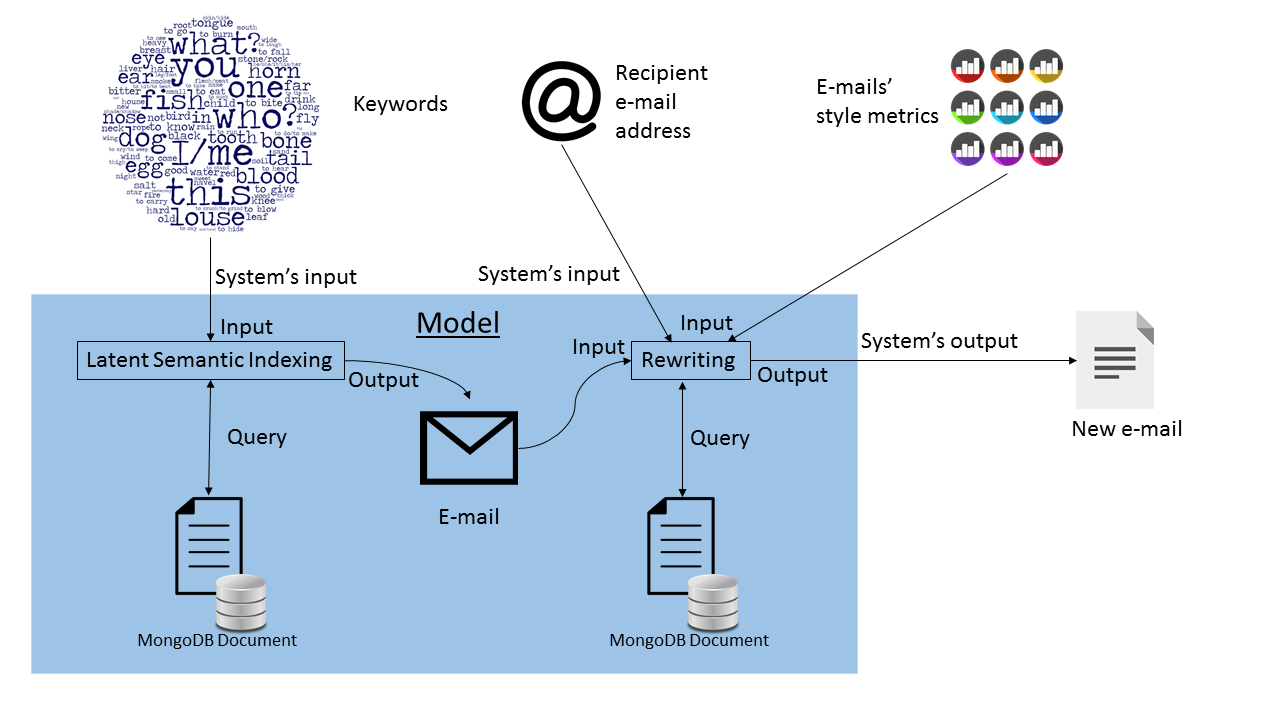
\includegraphics[width = 1.2\textwidth]{Imagenes/Bitmap/model.png}}%
	\caption{Model Architecture Diagram}%
	\label{fig:modarch}
\end{figure}

As we can see in Figure \ref{fig:modarch}, one of the required inputs of our system is the set of evaluated e-mail style metrics. Therefore it will be necessary to make use of the Analyser developed. As we have underlined, the modification of the given implementation depends on the purpose. It would be possible to remove the typographic correction phase if we want to develop a software aimed to be used by users (they will not have a good user experience if they have to correct their own e-mails before they can use the application) or if we want to take into account the typographic errors of the user with a new style marker. However, and thanks to the way the Style Analyser was implemented (with different modules as web services), any little or big modification in a module will not affect the rest of the phases. This will facilitate the reuse of the implementation developed. In this Section, we will not delve into it, instead we will just propose the model once the calculation of the different metrics is done.

Instead of trying to generate a complete e-mail, the basic idea of our model will be to rewrite one already written by the user. To achieve this, we design a model based on two phases: searching (its details are explained in Section \ref{sect:searchemail}) and rewriting (see Section \ref{sect:transemail}).

The searching phase is in charge of looking for a previously written message given a set of keywords. With this in mind, we can take advantage of the typographic corrected stored e-mails (or the preprocessed messages if this module is not used) to carry out the search. The only input that this module needs is the mentioned set of keywords, and its output is the text of the message written by the user.

The rewriting phase receives the output of the searching module. However, it will require more information in order to modify the text. For this reason, it is necessary to know who is going to be the recipient of the message and the results of the calculation of the style metrics. Once we know it, we can query the database where the classification of the different contacts is stored and, with this information, we are able to categorise the given contact. Its category will allow us to know the values of the style metrics of it and, with this information, we can choose the different methods to modify the e-mail. The output of the rewriting phase will be the new text of the message.

After having this brief introduction to the two different phases of our model, we can clearly know its inputs and outputs. At least it will be necessary to receive as input a set of keywords that describe the content of the message to be generated and its recipient. In addition we must have the style metrics previously calculated and the databases that store the texts of the messages and the established classification.

In respect of the output, it will be the generated text which is going to be the body of the e-mail sent to the given contact. Below we will detail each of the two phases that make up our system.

\section{Searching for the e-mail with the most similarity}\label{sect:searchemail}
The searching phase is in charge of finding the message in which the given set of keywords has the most weight. As we have studied in Section \ref{sect:lsi}, a good method used for this type of purposes is Latent Semantic Indexing. With it, we not only take into account the most significant words (eliminating stop words) but also, thanks to the Singular Value Decomposition (see Section \ref{ssect:svd}), we achieve a relationship between the term and the concept it represents, that is, we are able to face semantic problems in the consultation of documents such as synonymy that produce irrelevant results in methods such as boolean keyword queries. In fact, several researchers, such as \cite{landauer1998learning}, have shown that there is a significant correlation between the way humans and LSI process different documents. Other researchers, such as \cite{bartell1992latent} and \cite{ding1999similarity}, have demonstrated that LSI is a useful solution for conceptual matching problems.

However, LSI is a technique that requires a lot of memory and processing power. Both the generation of the TF-IDF table (see Section \ref{ssect:tfidf}) and the truncation of the singular value matrix have an expensive algorithmic complexity. To alleviate this problem it is possible to pre-calculate both TF-IDF table and the truncation of the singular values matrix. This way, when the user performs a query it is only necessary to read from a file the result of these operations.

In order to calculate the TF-IDF table, we need to access the database where we store the last version of the messages from which the different metrics have been extracted. It will be necessary to analyse each of the different e-mails stored. To obtain the different TF-IDF vectors it is recommended to use the most frequent expression (as \cite{tang2014email} claim) to find this value given a $t$ term in a $d$ document of the $D$ document collection:

$$
tfidf(t,d,D) = \frac{f(t,d)}{\max\{ f(t,d):t\in d\}}\cdot\log\left(\frac{\lvert D\rvert}{\lvert \{ d\in D: t\in d\}\rvert+1}\right)
$$

Once we have the table, we calculate its Singular Value Decomposition and truncate the singular value matrix to reduce its size and achieve the semantic relationships between the terms we are looking for (as it is explained in Section \ref{ssect:svd}).

Finally, we will take the input given by the user as keywords to generate the text message and make a query comparing the similarity between each message and the words provided by the user (as we have explained in Section \ref{ssect:query}). The output of the system will be the e-mail with the most similarity with all its information as the recipient and body of the message.

\section{Transforming e-mail according to metrics}\label{sect:transemail}
The rewriting phase will be responsible for modifying the message, obtained by the search phase, as necessary so that it has the style corresponding to the final recipient of the e-mail. To achieve this, we will need to know the category to which the person who will receive the message belongs. For this purpose, we will consult their e-mail address in the database where we can find the classification of the different contacts. In case no information is found about the consulted address, it will be necessary for the user to provide the category to which he or she belongs. As we will explain, this system requires to have previously data (written e-mails from which their style metrics have been extracted) of the category to which the recipient belongs, which can be a problem in case we consider writing a message destined to a new category.

As we have explained (see Chapter \ref{cap:analysis}), there are eight style metrics of the initial twenty-eight that best describe the writing style depending on the recipient of the message. These style markers are: \textit{verbAdjectiveRatio} (it is obtained by dividing the number of verbs by the number of adjectives), \textit{detPronRatio} (it is obtained by dividing the number of determinants by the number of pronouns), \textit{meanSentLen} (it is the average sentence length in word count), \textit{meanWordLen} (it is the average word length in number of characters), \textit{richnessYule} (it depends on the diversity of words, i.e. the number of different words and the number of words we do not repeat or appear twice, three, etc.), \textit{difficultyLevel} (it depends on both the percentage of words with one or two characters and the \textit{meanSentLen}), \textit{stopRatio} (it is the percentage of stop words) and \textit{entropy} (it depends on the number of times the same word appears). The modification of the e-mail will be based on trying to vary the value of these features according to the category to which the recipient belongs. In this way, we will obtain a message with values close to the averages of the style metrics of the category under consideration. There are several methods (with which we must assume that the message generated may not be correct due to issues such as polysemy and concordance in gender and number, among others) to modify them:

\begin{itemize}
	\item \underline{Change the number of adjectives}: removing adjectives is a simple task to perform and, except in cases where the adjective differentiates one entity from another, it does not cause problems when modifying the text. However, adding them is slightly more complicated. For this purpose, we could use a corpus of n-grams (like the Google n-grams\footnote{\url{http://storage.googleapis.com/books/ngrams/books/datasetsv2.html}}) to write the adjective that most commonly accompanies the noun at hand. Another way to address this problem is to add the adjectives according to the frequency with which the user uses them (using techniques such as probabilistic grammars used by \cite{halliday2014corpus}) making use of the stored messages. The disadvantage of the latter method is that it requires a large number of e-mails and with one as small as ours, it is likely that good results would not be obtained. On the other hand, this solution guarantees the use of the user's \textit{lexicon} (set of words used). The modification of the number of adjectives, will allow us to vary the following style metrics: \textit{verAdjectiveRatio} (although changing the number of verbs can be a complex task and we can find many problems, as we have seen, changing the number of adjectives is feasible), \textit{menaSentLen}, \textit{difficultyLevel} (as it affects the average length of sentences), \textit{richnessYule} (as it depends on the number of different words and the amount of times each word appears), \textit{stopRatio} (as it adds or removes adjectives, the percentage of stop words will be modified) and \textit{entropy} (changing the number of words in the text also changes the probability of each word appearing).
	
	\item\underline{Substitute words for synonyms}: Although we may make mistakes in cases such as polysemic words, replacing words with their synonyms would allow us to increase or decrease the value of some style metrics. To obtain the corresponding synonyms there are many web services\footnote{such as \url{https://holstein.fdi.ucm.es/nil-ws-api/}} or corpus from which we can extract them. Besides, we can use our bag of words (\textit{wordsAppearance} style marker) in order to use synonyms which belong to the user's \textit{lexicon}. The style metrics that would change their value with this method would be: \textit{meanWordLen} (it is possible to replace some words with longer or shorter synonyms to modify this feature), \textit{difficultyLevel} (as it also depends on the number of words in a syllable, although in our implementation it is the number of words with one or two characters, the replacement by synonyms of greater or lesser length can vary this descriptor), \textit{richnessYule} and \textit{entropy} (if a word is replaced by a synonym, its probability of occurrence decreases and that of the synonym used increases).
	
	\item\underline{Change the number of adverbs}: the elimination of adverbs may not be as easy as in the case of adjectives, as these express circumstances, such as mode, place, time, quantity, affirmation, doubt, etc. Nevertheless, it is possible to add or remove adverbs of quantity or similar (such as very, little or quite). To carry out this task we can use the same methods we used with adjectives: corpus of n-grams or reusing the ones written by the user in the analysed e-mails. This modification of the text would affect the following metrics: \textit{meanSentLen}, \textit{difficultyLevel}, \textit{richnessYule}, \textit{stopRatio} and \textit{entropy}.
	
	\item\underline{Change the number of pronouns}: When trying to remove or add pronouns we will be faced with the problem of co-reference, which consists of knowing to which entity each of the pronouns in the text refer. Nowadays we find some models to solve this challenge with quite promising results. The solutions use all kinds of techniques, such as the neural net scoring model that spaCy has\footnote{\url{https://spacy.io/universe/project/neuralcoref}} (which is an implementation of the study of \cite{clark2016deep}). Replacing an entity with a pronoun (i.e. reducing the number of pronouns) is not a complicated task, it just requires taking into account parameters, such as gender or number, that are offered by syntactic analysers such as spaCy. On the other hand, the opposite task involves the co-reference problem mentioned. One possible solution is to use existing complex systems such as the one we have presented. Another possibility is to take advantage of the characteristics of e-mails to obtain co-reference results to text pronouns. As e-mails are not very complex texts and do not usually involve many entities, it is possible to obtain a large percentage of successes by looking for nouns that have the same number and gender and staying with the most numerous or the closest to the pronoun. In any case, the modification of the number of pronouns in the text would affect the following style metrics: \textit{detPronRatio}, \textit{meanSentLen}, \textit{stopRatio}, \textit{difficultyLevel}, \textit{richnessYule} and \textit{entropy}.
\end{itemize}

With these modifications of the original message, it will be possible to bring its style metrics closer to the desired value. However, it is necessary to underline that each one of these affects more than one style markers, which means that we are significantly varying the value of more than one metric. In the presentation of this model, we are assuming, as the logic indicates, that all these descriptors are slightly correlated, either in directly or inversely proportional way. Nevertheless, we run the risk of making use of one of the four previous changes and approaching the desired value of a feature while we are moving away from the mean of other style metric.

If we are able to change the values of the eight chosen style markers to its corresponding mean according to the category of the contact, we will have a text of the personalised message based on the recipient as we wanted to obtain.